\section{Results}
\label{sec:results}

\begin{figure*}[ht]
    \centerline{\framebox{
    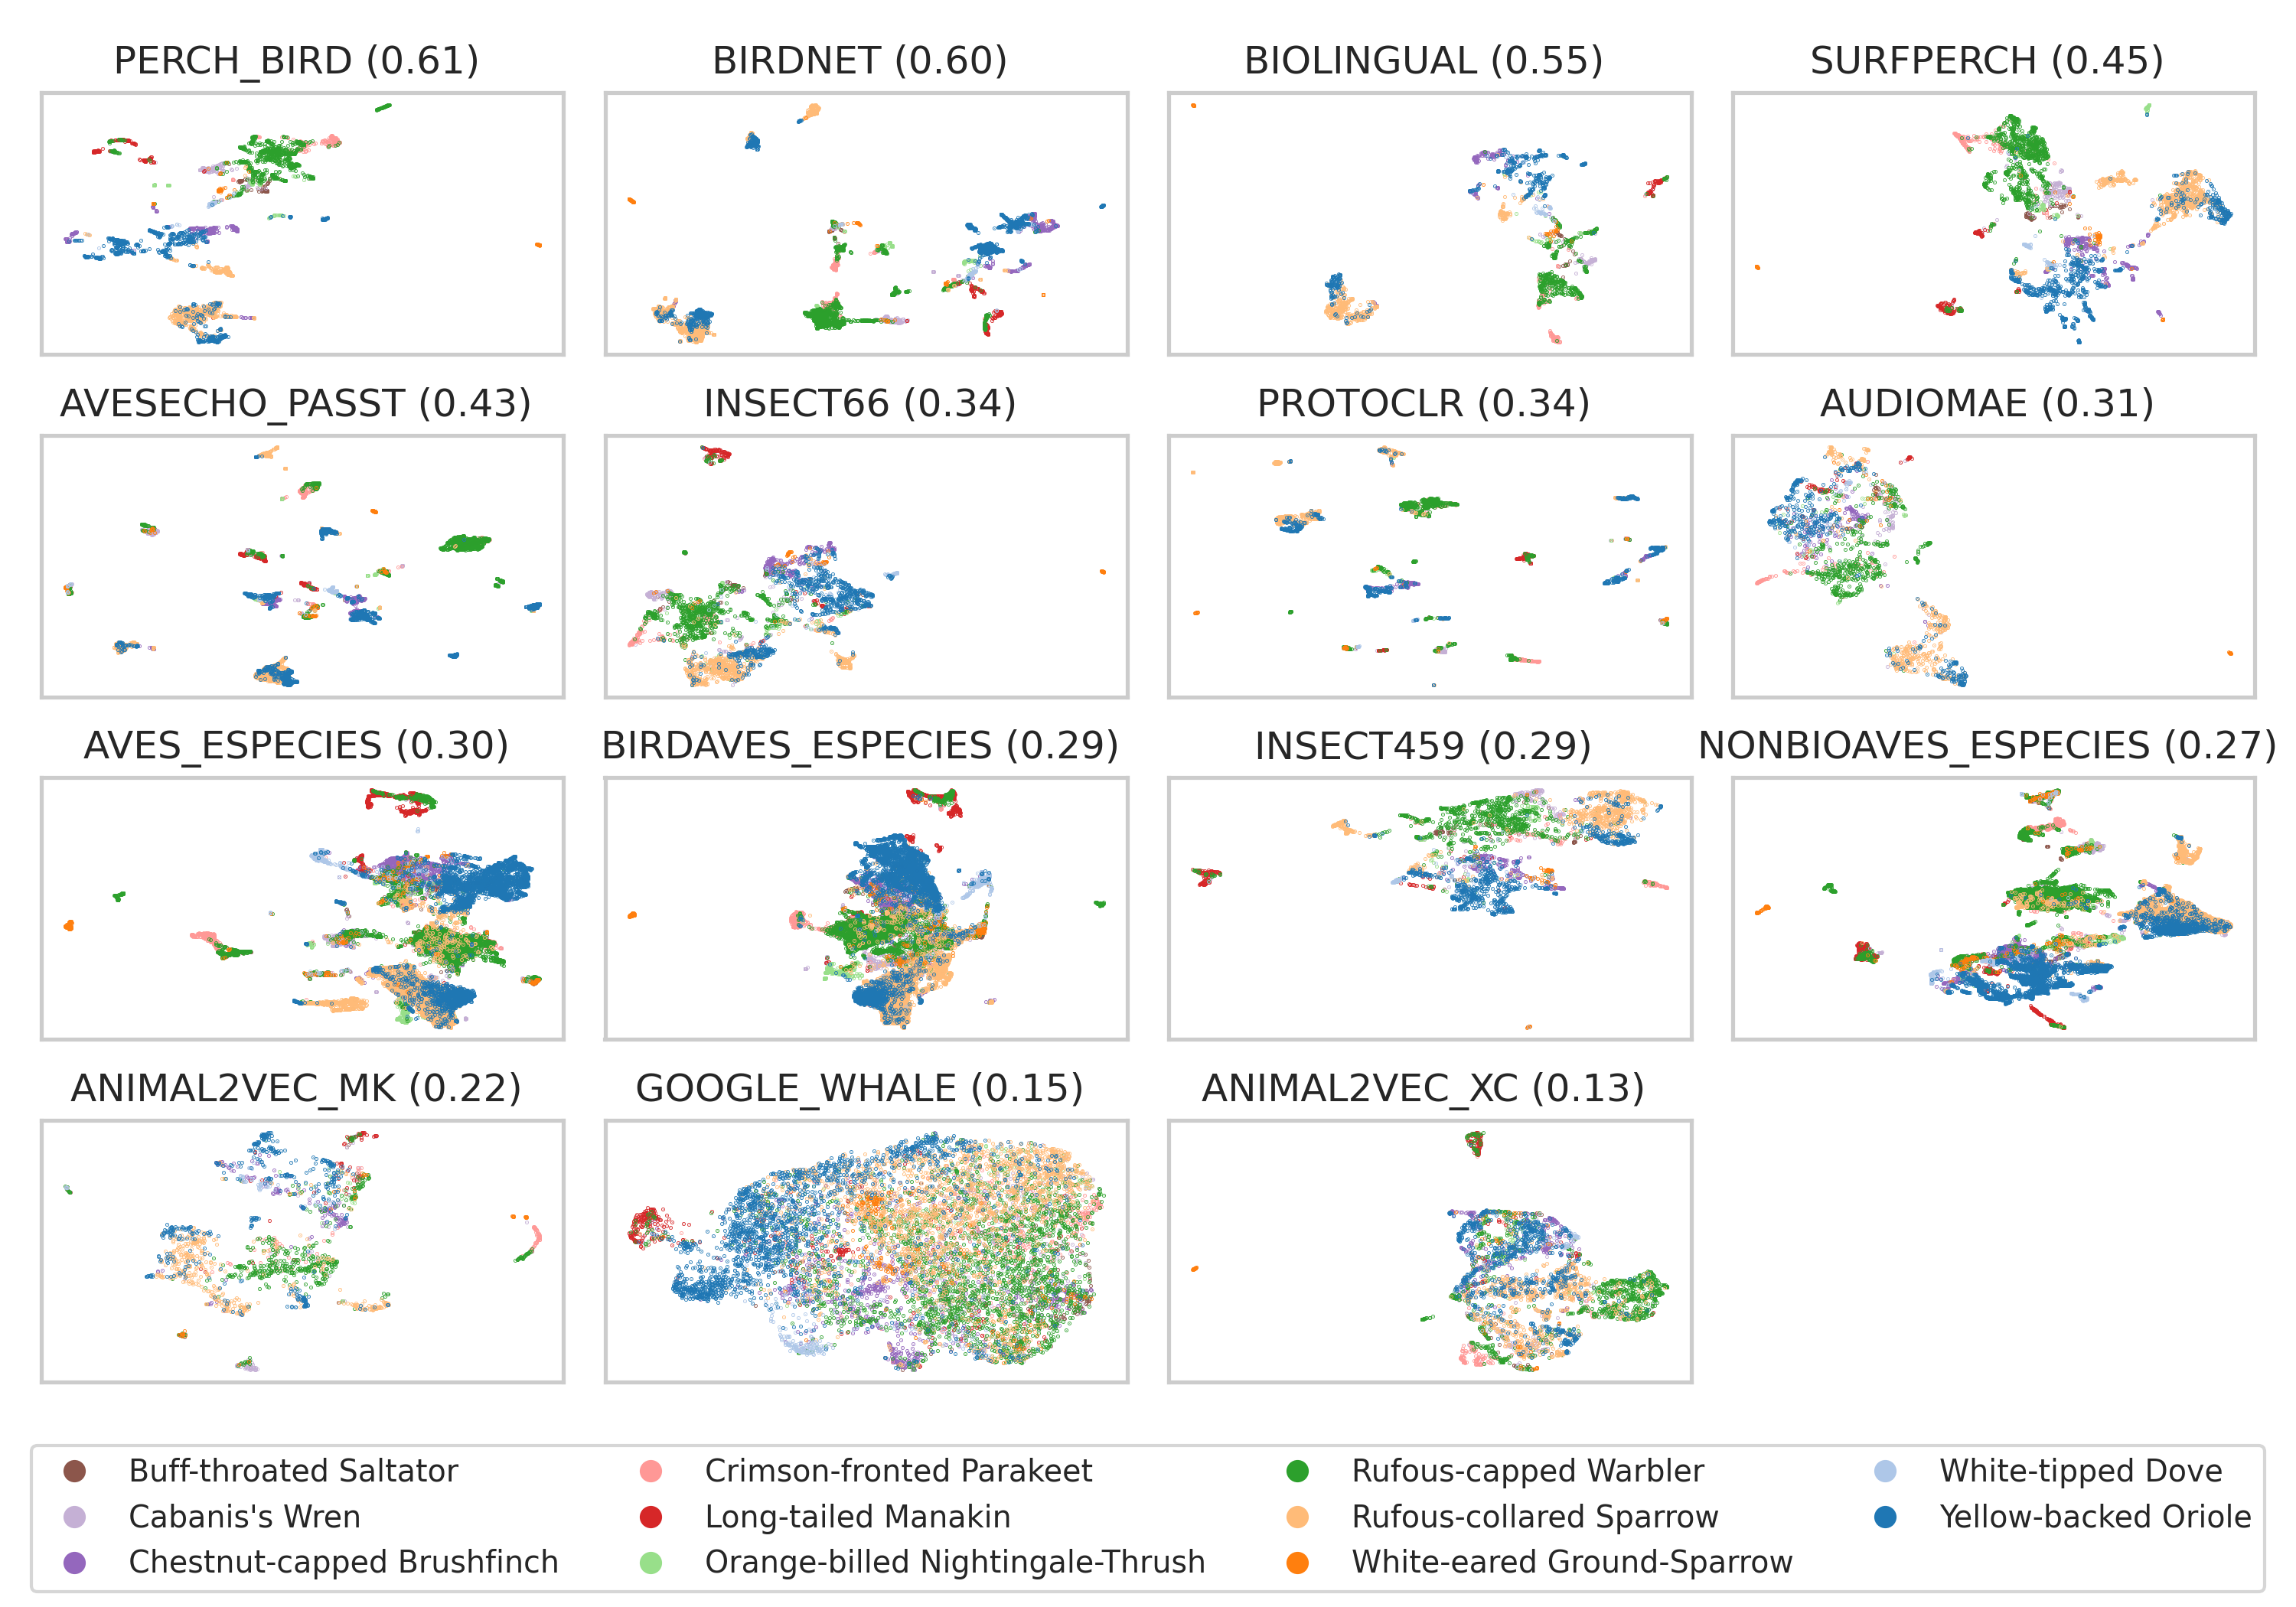
\includegraphics[width=16.3cm]{Sections/imgs/normal_overview.png}}}
    \caption{Two-dimensional embedding spaces of all feature extractors, sorted descending by their clustering performance of AMI values (indicated next to their name) from top left to bottom right.
    Given the different input lengths of the feature extractors, the number of embeddings vary significantly.
    Colors correspond to the class labels, which are 11 different tropical bird species.}
    \label{fig:embeds}
\end{figure*}

% Embeddings spaces of are visualized using UMAP in are generated from the input data using all feature extractors and then the dimensionality reduction algorithm UMAP is used to visualize the data in two dimensions.
% The results are shown in Fig. \ref{fig:embeds}.

Two dimensional UMAP embeddings are shown in Fig. \ref{fig:embeds}.
The worst performing feature extractors, produce large unstructured clouds of mixed color, indicating that no significant clustering is achieved.
In the first and second row, feature extractors can be seen to separate the embeddings into meaningful clusters.
It is noticable that some feature extractors such as AvesEcho\_PaSST and ProtoCLR seem to generate more subclusters than most other feature extractors.
The seven best performing feature extractors are all trained using supervised learning and the top three additionally trained on bird vocalizations.
All three of the AVES models (BirdAVES, AVES and NonBioAVES) reach similar performances in spite of big differences in their fine-tuning datasets \cite{hagiwara_aves_2022}.

\begin{figure}[ht]
    \centerline{\framebox{
        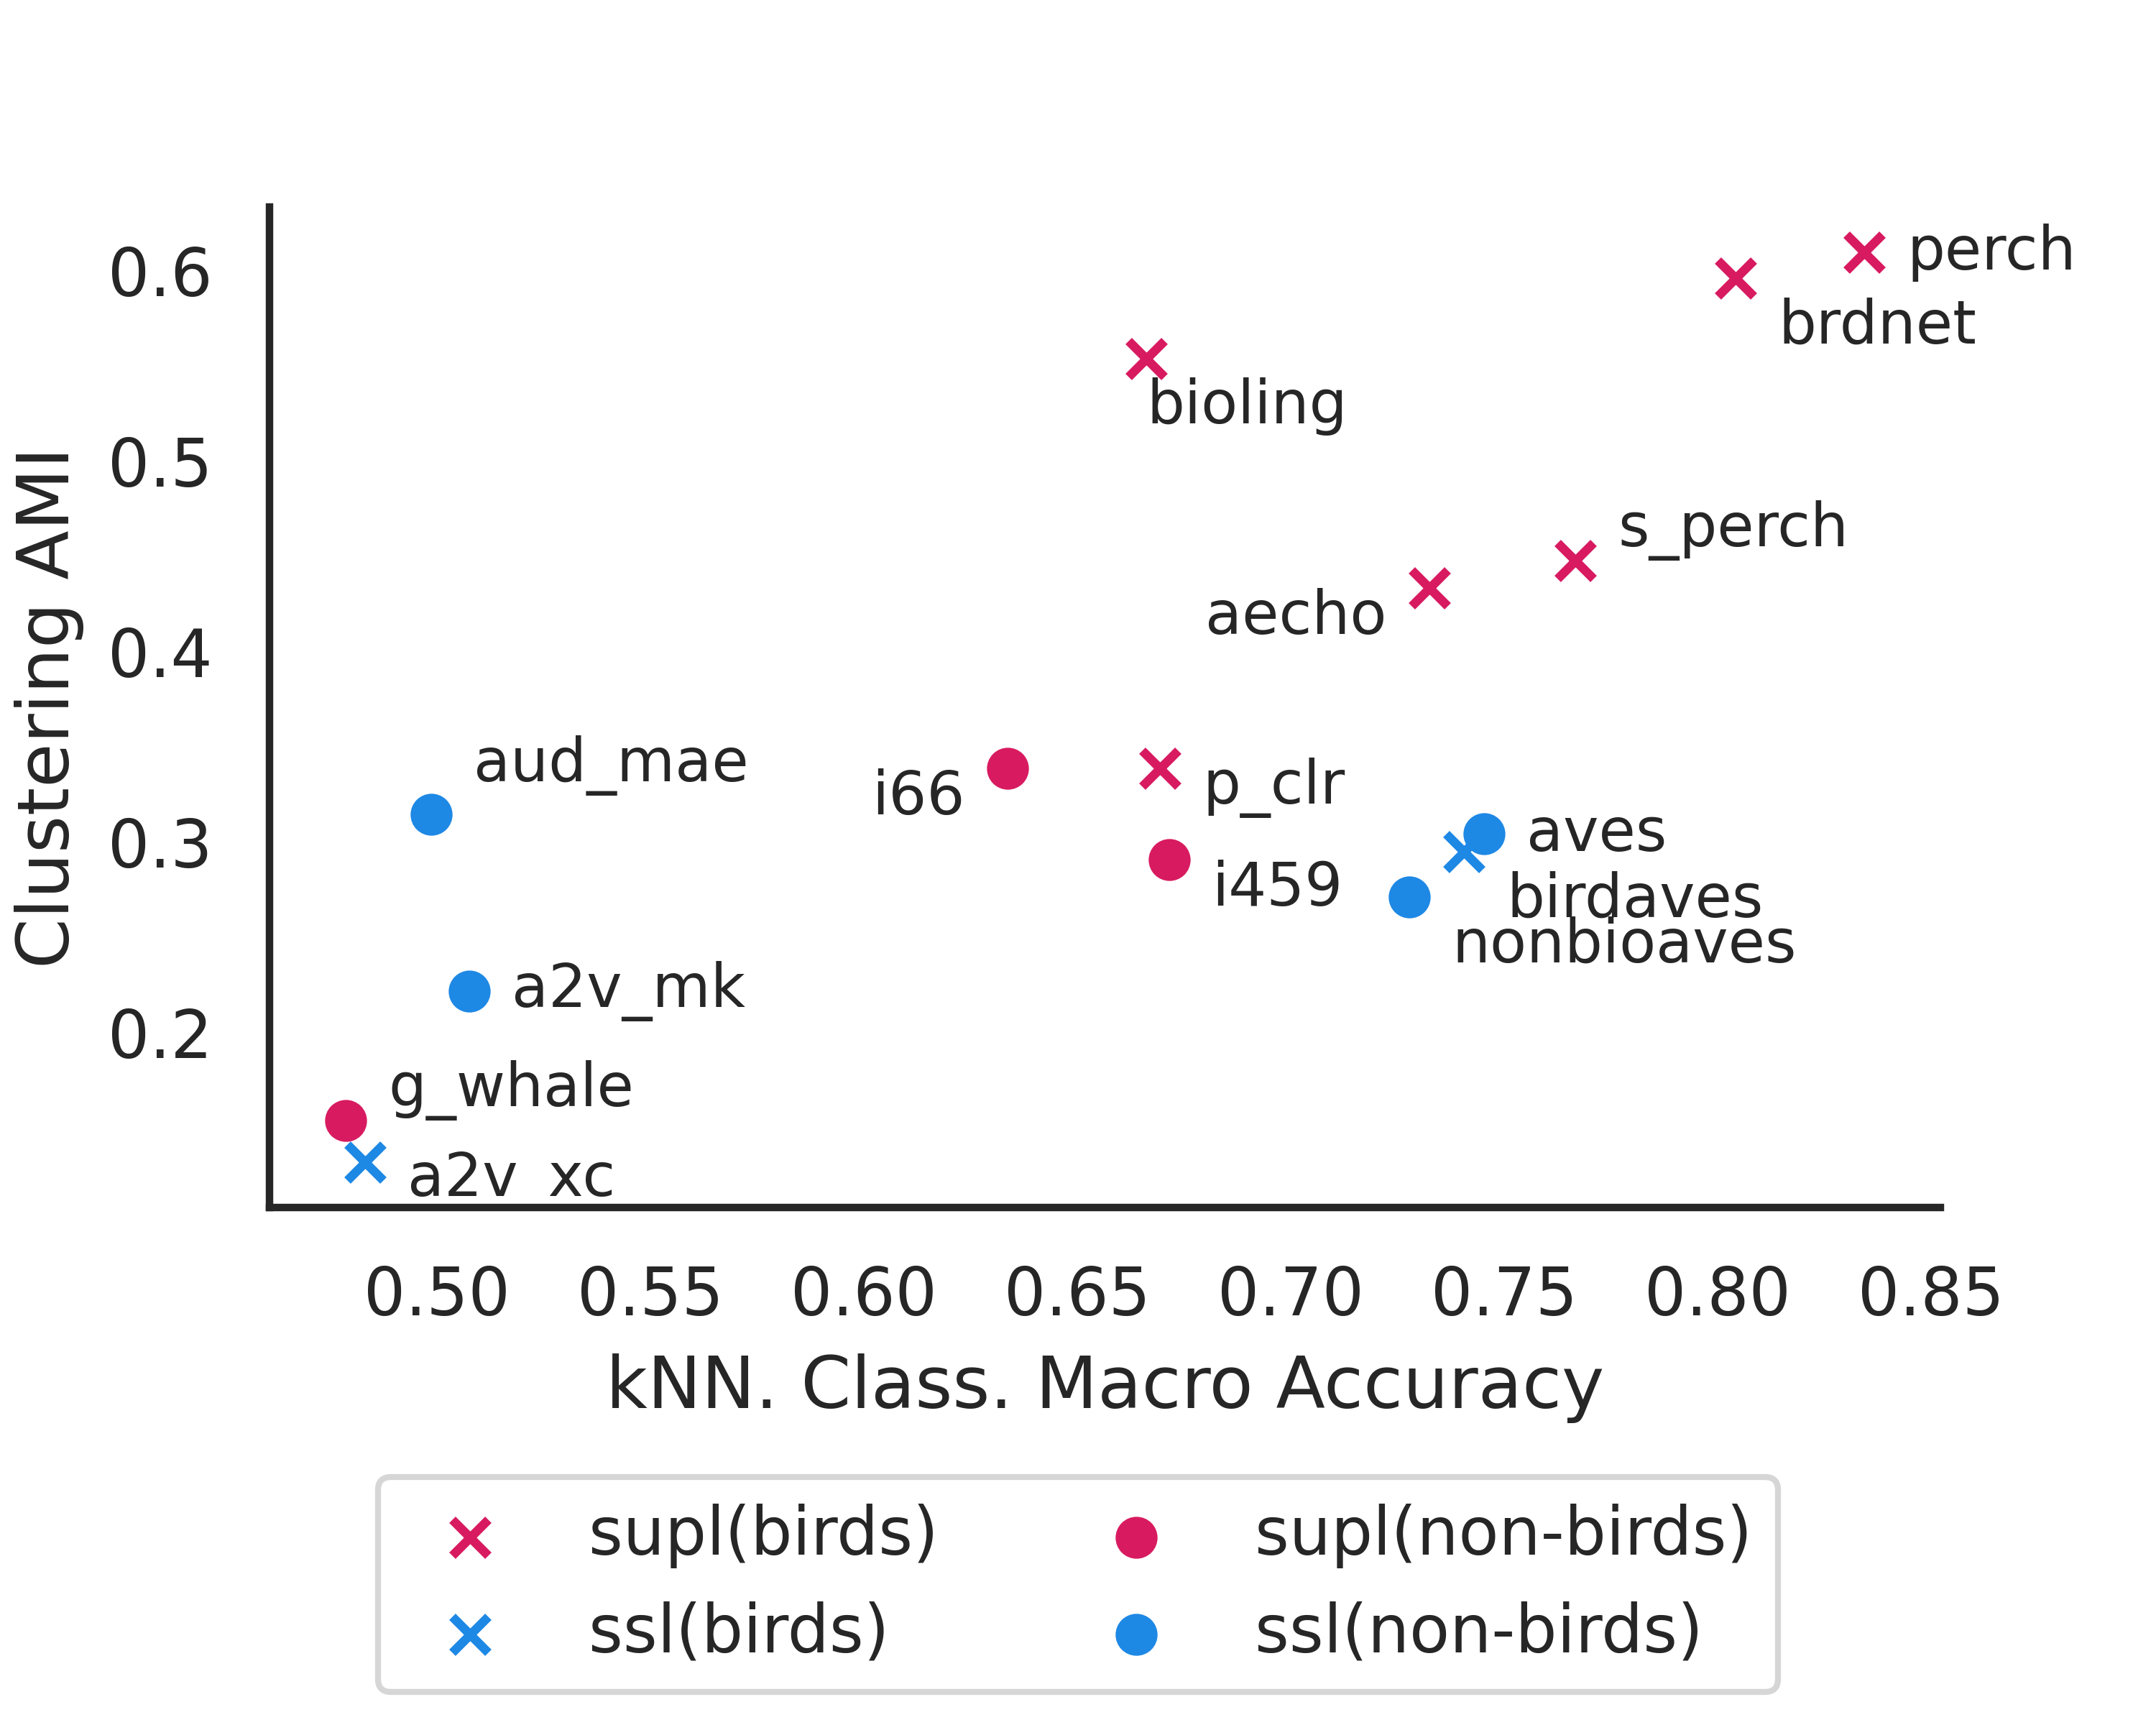
\includegraphics[width=7.8cm]{Sections/imgs/scatterplot_clust_vs_class_nt_knn_normal.png}}}
        \caption{Comparison of feature extractors by learning paradigm and training data. Abbreviated names correspond to abbrev. column in Tab. \ref{tab:bacpipe_models}. Differences in color correspond to training paradigm and differences in symbols correspond to training data. The x-axis shows clustering results of AMI while the y-axis shows macro accuracy results of linear classification. Colors correspond to supervised learning and self-supervised learning feature extractors, while symbols separate bird and non-bird training data.}
        \label{fig:subl_vs_ssl}
    \end{figure}
    
To investigate how training setup and training data affect performance, Fig. \ref{fig:subl_vs_ssl} shows a scatterplot of the different feature extractors.
Performance is evaluated by macro accuracy of linear classification on the x-axis and AMI of clustering on the y-axis.
% AMI is chosen to evaluate clustering performance as we are primarily interested to see how well the KMeans clustering agrees with the ground truth.

When focussing on the y-axis, all self-supervised learning feature extractors (in red) reach clustering performances under 0.31.
Performance by linear classification is more equally distributed, however, again supervised learning feature extractors reach the three highest values.
Furthermore, Animal2vec\_XC, the only self-supervised learning feature extractor that was not fine-tuned, performs poorly by both clustering and linear classification.
Google\_Whale represents the only supervised learning feature extractor performing very poorly by clustering.

Comparing by training data, feature extractors trained on only or including bird datasets outperform the other feature extractors by linear classification and even more so by clustering.
When looking at the combined performance by clustering and linear classification, Animal2vec\_XC and ProtoCLR are the only two feature extractors trained on birds that perform poorly.
Biolingual, which was trained on large bird databases using a multi-modal approach performs well by clustering, but poorly by linear classification.

When referring back to Table \ref{tab:bacpipe_models} embedding dimension does not correlate with clustering or linear classification performance.
Furthermore, the only two feature extractors trained on marine sounds, Google\_Whale and SurfPerch (trained on birds and marine sounds) reach very different performances.
    
\begin{figure}[ht]
    \centerline{\framebox{
    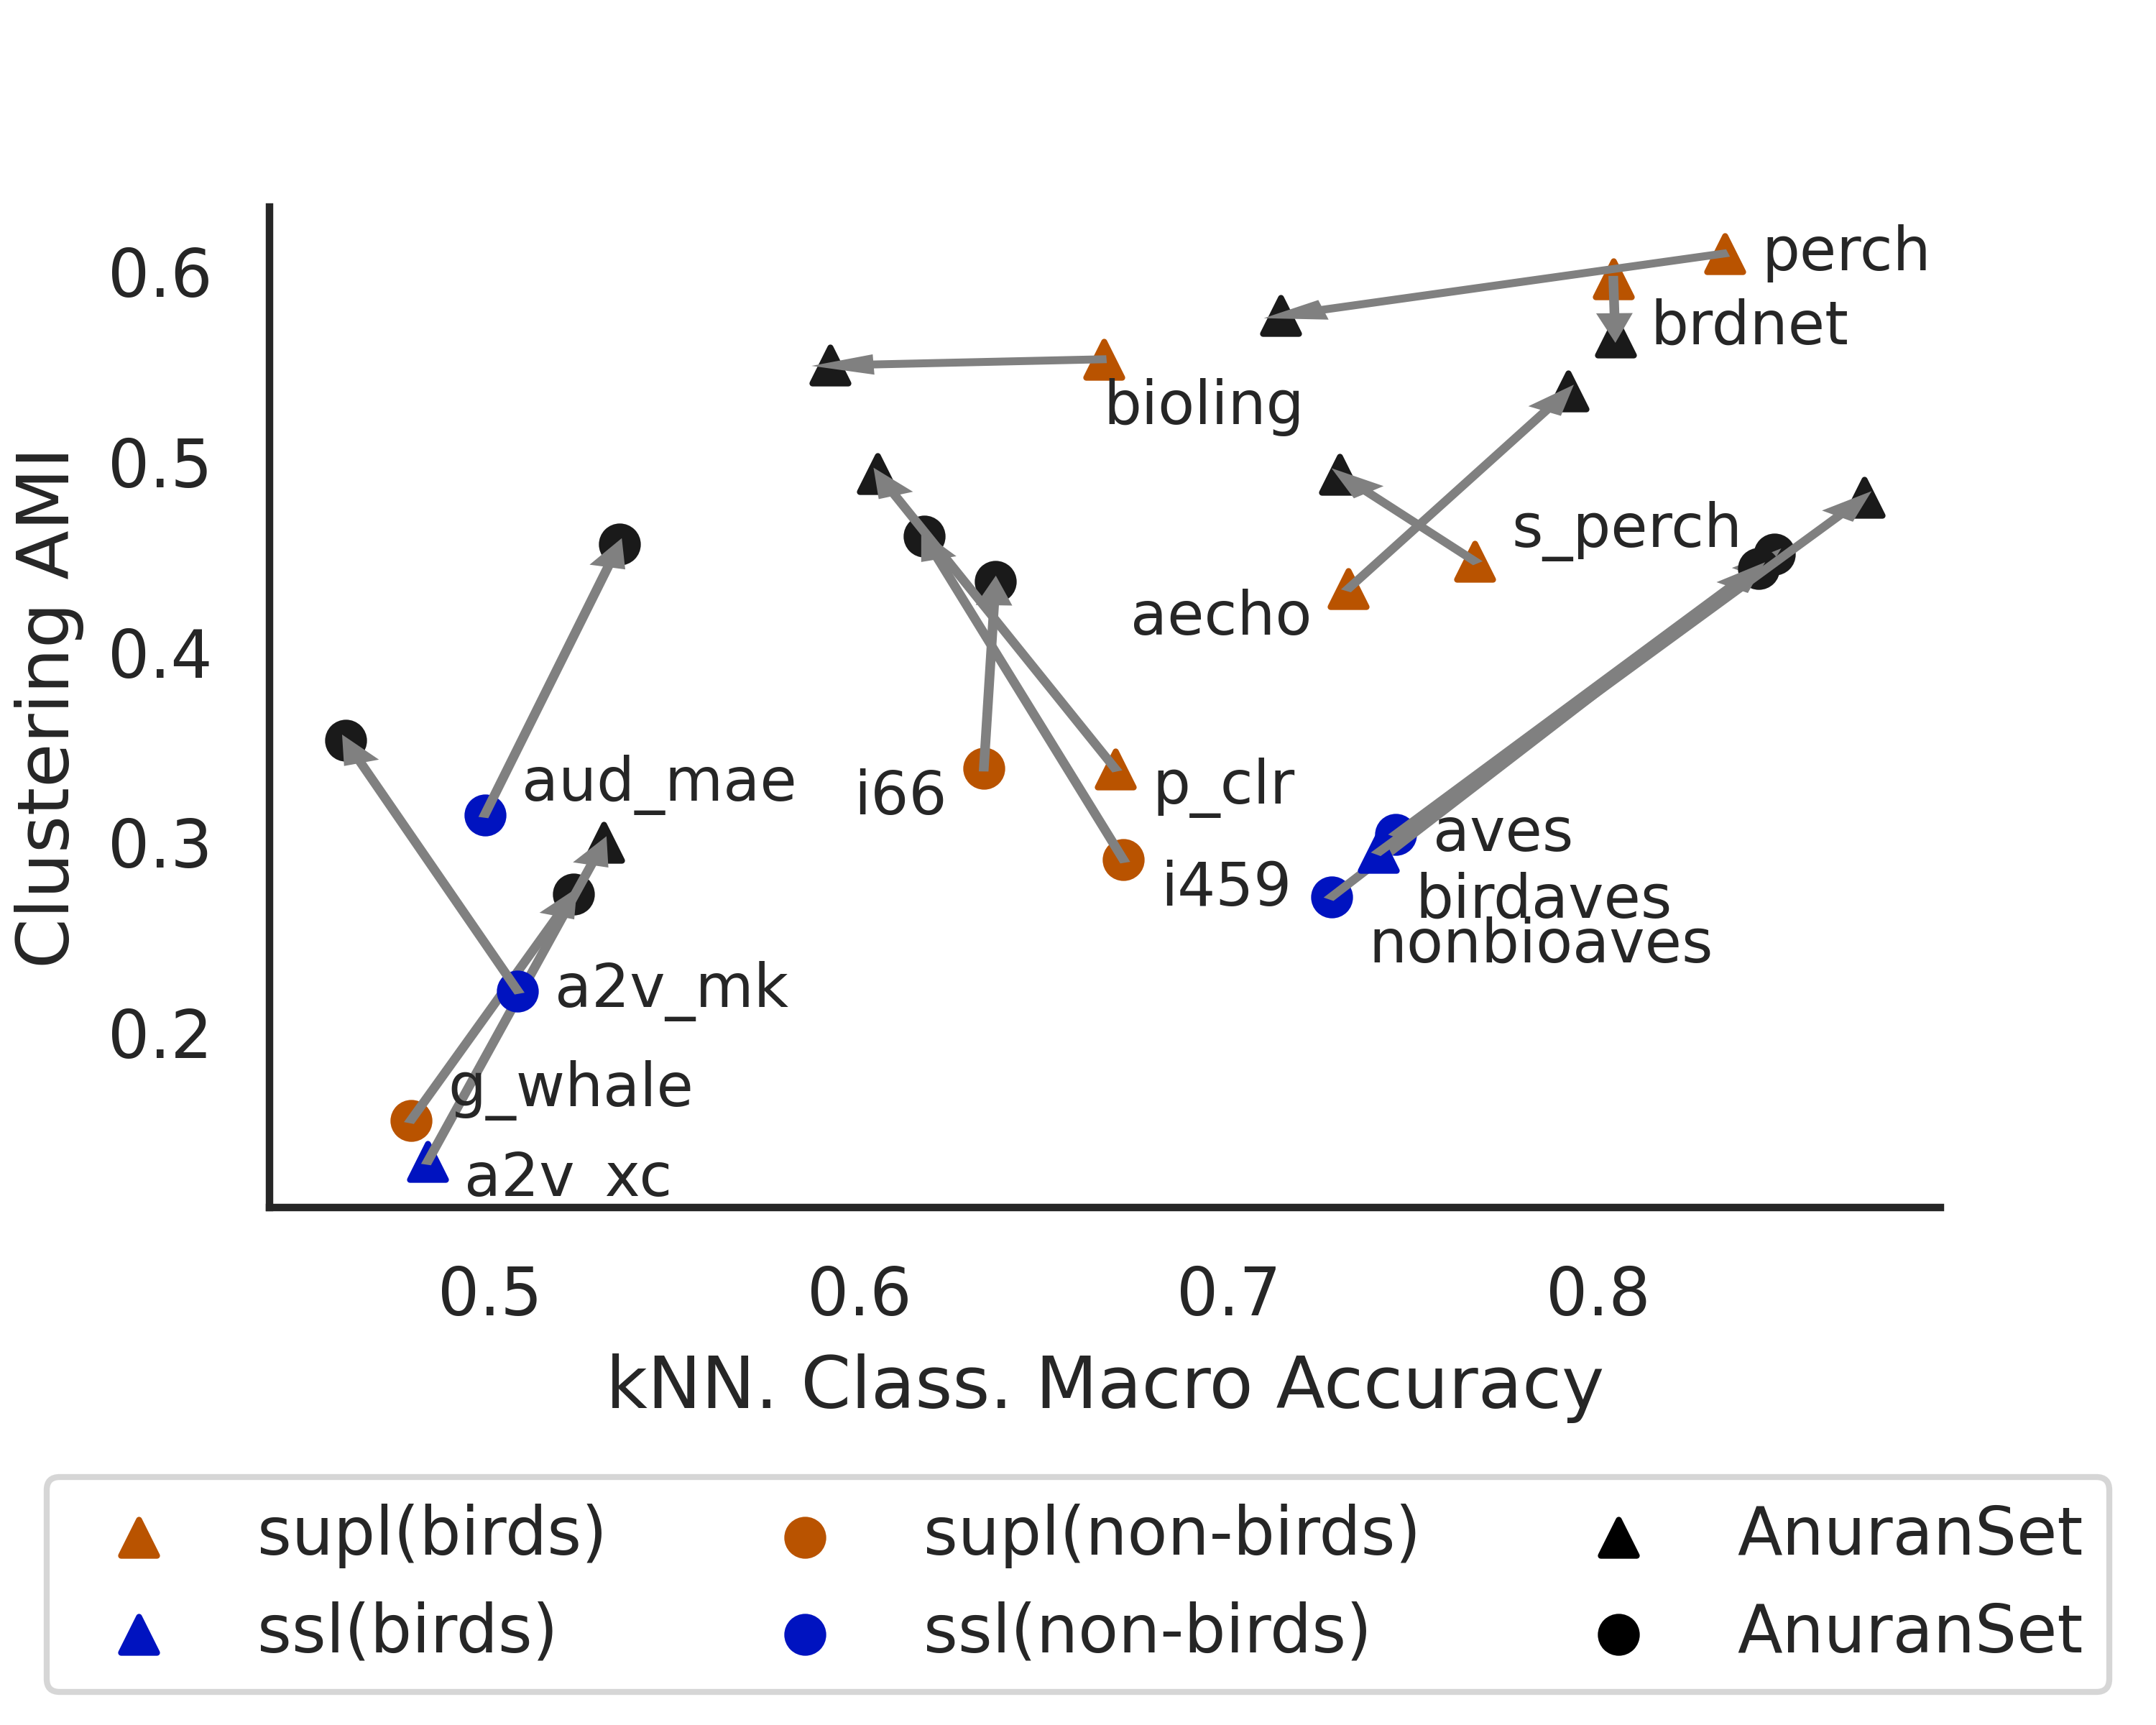
\includegraphics[width=7.8cm]{Sections/imgs/scatterplot_clust_vs_class_neotrop_anuran_normal.png}}}
    \caption{Comparison of feature extractor performance in original high dimensional embedding space and reduced 300 dimensional space using PCA. 
    The x-axis shows clustering results of AMI while the y-axis shows macro accuracy results of linear classification. 
    Symbols denote supervised or self-supervised learning, while red and green correspond to bird and non-bird training data. 
    The grey line and black markers indicate performance in the reduced dimensional embedding space.}
    \label{fig:orig_vs_ump}
\end{figure}

To account for the differences in embedding dimension, we visualized the change in performance between the original embedding space and a standardized embedding dimension of 300, to which all embedding spaces were reduced to using PCA.
The results are shown in Fig. \ref{fig:orig_vs_ump}.
While the poorly performing models ProtoCLR and Animal2vec\_MK are able to increase their linear classification performance, Insect459, Insect66 and Google\_Whale slightly improve linear classification and clustering performance.
While linear classification performance remains similar, SurfPerch, BirdNET and AvesEcho\_PaSST all decrease in clustering performance.
For the remaining feature extractors, standardizing the dimension, does not affect performance significantly.